\lhead{\emph{Histogram}}
\chapter{Histogram}

In this section, we will delve into the implementation details of histograms and explore various operations such as insertion, update, and deletion. Understanding these fundamental aspects will provide you with a comprehensive understanding of how histograms are built and manipulated.

\section{Implementation Details}
\subsection{The Insertion Algorithm}


\begin{figure}[H]
    \centering
    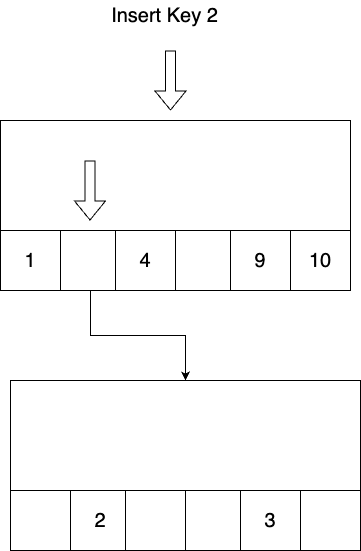
\includegraphics[width=50mm,scale=1]{Figures/InsertionHist.png}
    \caption{
     Example of Histogram Insertion
    }
    \label{fig:HistInsertionExample}
\end{figure}

The strategy we employ for the insertion of histograms is very similar to that of the baseline strategy. However, there are some noteworthy differences in the way we rebuild nodes. Rather than relying on the traditional methods, we use a histogram approach to obtain an approximate distribution of the data. This allows us to generate keys, denoted by $x$, and their corresponding positions or labels, denoted by $y$.

To further refine the model, we use Ordinary Least Square (OLS) to obtain the slope and y-intercept for linear regression. This aids in the accurate identification of conflicts within the data. The rebuilding process occurs when a new node has a depth that is at least twice that of the previous node, in a similar fashion to the baseline strategy.
\begin{algorithm}
\caption{Histogram Insertion}
\begin{algorithmic}[1]

\Procedure{insert}{node, key}
\State $current\_node \gets node$
\State $path\_size[]$
\While{$node \neq null$}
\State $pos \gets PREDICT\_POS(current\_node, key)$
\If{$pos$ is child node}
    \State $current node \gets node[pos]$
    \State $path\_size[i] \gets node$
\Else
    \State $key\_pos = PREDICT\_POS(current\_node, key)$
    \State $node[key\_pos] \gets key$
    \State update $frequency\_array$
\EndIf
\EndWhile
\For{$i \gets 0$ to $path\_size - 1$}
   \State $node \gets path[i]$
    \If{rebuilding criteria}
        \State $keys \gets collect\_keys$
        \State $new\_node \gets rebuild\_tree$
        \State $path\_size[i] \gets new\_node$
    \EndIf
\EndFor

\EndProcedure
\end{algorithmic}
\end{algorithm}

In cases where conflicting elements arise, a new node is created to ensure the integrity of the data. However, the creation of new nodes comes with an additional computation, which slows down the insertion time. This is because the model needs to be trained to accommodate these conflicting keys and accurately insert them into the gapped array.

As an example in Figure \ref{fig:HistInsertionExample}, if a key $2$ is inserted into an existing tree, the predicted position will be $1$. However, $1$ is already occupied, so the tree will create a new node that contains $2, 3$ and replace the root node $pos[1]$ as the pointer pointing to the child node.

Overall, the insertion strategy for histograms relies on a combination of techniques such as the use of OLS and histogram analysis to ensure that the data is accurately represented and conflicts are resolved promptly. While it may result in slightly slower insertion times, the benefits of a more accurate representation of the data outweigh the costs.

\subsection{The Query Algorithm}

\begin{figure}[H]
    \centering
    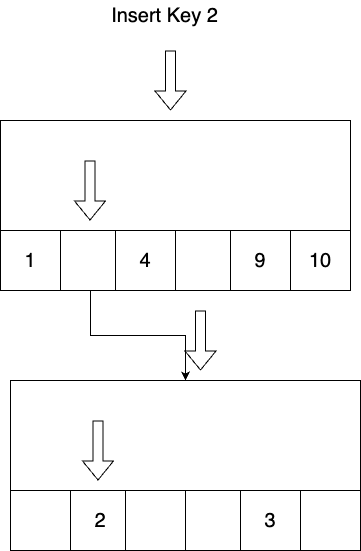
\includegraphics[width=70mm,scale=1]{Figures/QueryHist.png}
    \caption{
     Example of Histogram Query
    }
    \label{fig:HistQueryExample}
\end{figure}
To perform a search operation in \learnindex, the algorithm starts at the root node of the tree and traverses down to the leaf nodes to find the data. One of the advantages of \learnindex is that it uses a model-based insertion technique, which allows it to perform search operations efficiently. When there is a conflict during insertion, \learnindex creates a new child node rather than shifting the keys to the closest gaps. This ensures that there are no misplacement in the index, which can slow down search operations by making performing a search after traversing down the tree.

The search algorithm in \learnindex starts by pushing the root node into the stack. Using the current node's linear regression model, the algorithm predicts the position of the keys it is searching for. It then checks if the predicted position is a child or a key. If the predicted position is a child, the algorithm pushes the child node onto the stack and continues the search. If the predicted position is a key, the algorithm returns the key.
\begin{algorithm}
\caption{Histogram Query}
\begin{algorithmic}[1]
\Procedure{query}{node, key}
\State $current\_node \gets node$
\While{$node \neq null$}
\State $pos \gets PREDICT\_POS(current\_node, key)$
\If{$pos$ is child node}
    \State $current node \gets node[pos]$
    
\Else
    \State $key\_pos = PREDICT\_POS(current\_node, key)$
    \State \Return $node[key\_pos]$
\EndIf
\EndWhile
\State return null
\EndProcedure
\end{algorithmic}
\end{algorithm}

The child node continues to be pushed onto the stack until the algorithm reaches the node that contains the key it is searching for. This process allows for efficient search operations, as the algorithm only explores the parts of the tree that contain the key it is searching for.

As an example, in Figure \ref{fig:HistQueryExample}, if we perform a query after the insertion for a key $2$, the model predicts the location of key $2$ in location $1$ and it has to follow the pointer down to leaf node and use the model at leaf node to predict the location of key $2$.
\subsection{The Deletion Algorithm}


\begin{figure}[H]
    \centering
    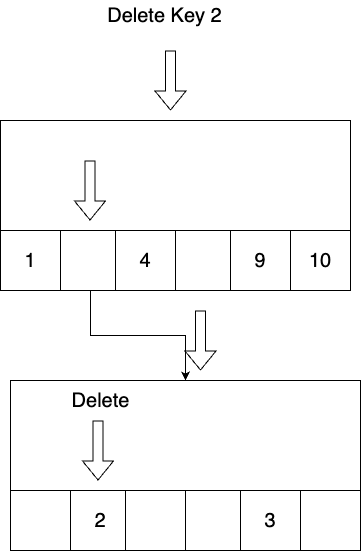
\includegraphics[width=70mm,scale=1]{Figures/DeleteHist.png}
    \caption{
     Example of Histogram Delete
    }
    \label{fig:HistDeleteExample}
\end{figure}
Deletion is an essential operation for any data structure that stores data, and \learnindex is no exception. Deletion in \learnindex follows a similar strategy as search, where the algorithm has to traverse down the tree until reaching the node where the key is located. Once the node is found, the key can be removed from the tree.
However, there is a critical difference between deletion and search in \learnindex. During deletion, the algorithm must also free up space in the gapped array, and also update the bitmap index that this position contains a gap instead of a key.

\begin{algorithm}
\caption{Histogram Delete}
\begin{algorithmic}[1]

% \State $\texttt{MAX_DEPTH} \gets 128$
\Procedure{Delete}{node, key}
\State $current\_node \gets node$
\While{$node \neq null$}
\State $pos \gets PREDICT\_POS(current\_node, key)$
\If{$pos$ is child node}
    \State $current node \gets node[pos]$
    
\Else
    \State $key\_pos = PREDICT\_POS(current\_node, key)$
    \State delete $node[key\_pos]$
    \State update $frequency\_array$
\EndIf
\EndWhile
\EndProcedure
\end{algorithmic}
\end{algorithm}
To perform the deletion, the algorithm starts at the root node and uses the same model-based approach to predict the position of the key. As the algorithm descends the tree, it checks each node's bitmap to determine whether the key is present in that node. Once the node containing the key is found, the key is deleted, and the algorithm updates the bitmap that stores it in the current node.

For an example Figure \ref{fig:HistDeleteExample}, deleting key $2$ requires traversing down from root node until reaching key $2$ nodes similar to query, then use the model to predict the location of key $2$ before deleting it from the gapped array.  

\subsection{The Range Query Algorithm}
\begin{algorithm}
\caption{Histogram Range Query}
\begin{algorithmic}[1]

\Procedure{range\_query}{root, lower, upper}
  \State $stack \gets \text{empty stack}$
  \State $current\_node \gets root$
  \State $keys \gets \text{empty array}$
  \While{$current\_node \neq \text{null}$ \textbf{ or } $stack$ is not empty}
    \While{$current\_node \neq \text{null}$}
      \State $\text{push } current\_node \text{ to } stack$
      \State $pos \gets \text{PREDICT\_POS}(current\_node, \text{lower})$
      \If{$pos$ is a child node}
        \State $current\_node \gets current\_node[pos]$
      \Else
        \State \textbf{break}
      \EndIf
    \EndWhile
    \If{$\text{stack}$ is not empty}
      \State $current\_node \gets \text{pop a node from } stack$
      \State $key\_pos \gets \text{PREDICT\_POS}(current\_node, \text{lower})$
      \For{$i \gets \text{key\_pos}$ to $\text{node\_size}-1$}
        \If{$\text{node}[i] \leq \text{upper}$}
          \State $\text{append } \text{node}[i] \text{ to } keys$
        \Else
          \State \textbf{break}
        \EndIf
      \EndFor
      \State $current\_node \gets current\_node[\text{next position}]$
    \EndIf
  \EndWhile
  \State \textbf{return} $keys$
\EndProcedure
\end{algorithmic}
\end{algorithm}

Range queries are an essential operation in \learnindex, particularly when dealing with sorted collections of keys. Such queries involve searching for a range of keys within a given dataset and are commonly used in a wide range of applications, including databases, search engines, and information retrieval systems.

One of the advantages of using a sorted dataset is that it makes range queries relatively easy to perform. By searching for the first key in the range and then iterating through the data structure to collect all keys until the end key is reached, the algorithm can efficiently retrieve all of the data within the specified range.


\subsection{The Adjustments Algorithm}

\begin{algorithm}
\caption{Histogram Gap Distribution}
\begin{algorithmic}[1]
\Procedure{Histogram Distribute}{node, keys, size, gap\_multiples}
 \State $\text{num\_bins} \gets 0$
  \State $\text{bin\_size, bin\_width} \gets node.hist$
  
  \State $\text{total\_gaps} \gets \text{round}(size \times \text{gap\_multiples})$
  
  \State $\text{gaps\_per\_bin} \gets \text{empty vector}$
  \State $\text{sum\_counts} \gets 0$
  
  \For{$i \gets 0$ to $\text{num\_bins} - 1$}
    \State $\text{gaps} \gets \text{round}(bin\_size \times \text{total\_gaps} / size)$
    \State $\text{gaps\_per\_bin}.\text{push\_back}(\text{gaps})$
    \State $\text{sum\_counts} \gets \text{sum\_counts} + bin\_size$
  \EndFor
  
  \State $\text{result} \gets \text{empty array of size} \ 2 \times size$
  \State $\text{min\_val} \gets \text{keys}[0]$
  \State $\text{outSize} \gets 0$
  
  \For{$i \gets 0$ to $size - 1$}
    \State $\text{bin\_index} \gets \text{floor}((\text{keys}[i] - \text{min\_val}) / \text{bin\_width}$
    
    \State $\text{result}[\text{outSize}] \gets \text{keys}[i]$
    \State $\text{outSize} \gets \text{outSize} + 1$
    
    \If{$\text{hist.first}[\text{bin\_index}] > 0$}
      \State $\text{result}[\text{outSize}] \gets 0$
      \State $\text{hist.first}[\text{bin\_index}] \gets \text{hist.first}[\text{bin\_index}] - 1$
      \State $\text{outSize} \gets \text{outSize} + 1$
    \EndIf
  \EndFor
  
  \State \textbf{return} \text{result}
\EndProcedure
\end{algorithmic}
\end{algorithm}
The strategy we employ to make adjustments to the \learnindex structure utilizes the same condition as \acrshort{lipp}. Prior to making any adjustments, our algorithm traverses the data structure and collects the keys that will be involved in the adjustments. We then create a new node to store these keys. 

However, our approach differs in the way we analyze the collected data. Rather than using \acrfull{fmcd}\cite{LIPP}, we use a histogram to examine the distribution of the data and select a bin width based on the characteristics of the collected data.  By doing so, we are able to make more informed decisions about the optimal size of the bin width, which can ultimately lead to more efficient and effective adjustments to the \learnindex.




\section{Theoretical Analysis}
When inserting a node into a gapped array, the algorithm must traverse down the tree until it finds an empty gap to fill. This process takes $O(\log N)$ time.

However, the linear regression model used to predict the position of keys is much more efficient, taking only $O(1)$ time due to its reliance on simple multiplication operations. Additionally, when a new node is inserted into the tree, the histogram in each node must be updated to reflect the new frequency of data points.

To accomplish this, we use an array of frequencies and calculate the bin index using the formula $bin\_index = floor((data\_point - min\_value) / bin\_width)$. The calculation of the bin index for a single data point takes only $O(1)$ time due to the simplicity of the arithmetic operations and the use of the floor function. However, insertions need to be readjusted when the condition is met, similar to the \acrshort{lipp} index, which will cost $O(N\log N)$ where N is the number of keys in the tree. In adjustments, gap redistribution is required and retrained the model to get the accurate prediction of keys and location. However, the adjustments do not occur every time we traverse down the tree path. In this case, we can amortize the cost such that we save $\log N$ credit every time we pass a path which makes the insertion costs similar to the baseline, which is $O(\log^2 N)$

However, the time complexity for updating the histogram frequency with bin width using an array varies depending on the number of data points that map to the same bin. In the best case, the time complexity for updating the frequency is $O(1)$, as updating an element in an array takes constant time. However, in the worst case, the time complexity for accessing the frequency element is $O(\epsilon)$, where $\epsilon$ is the number of data points that map to the same bin. This is because computing the index to access the array element can require linear time.

Therefore, the efficiency of updating the histogram frequency in each node during the insertion process can vary greatly depending on the number of data points that map to each bin. However, the overall time complexity of inserting a new node into the gapped array is dominated by the traversal down the tree, which takes $O(\log N)$ time.

However, deleting a key in the \learnindex algorithm involves more than just traversing down the tree. Once the key is located, the algorithm needs to perform deletion and free the memory in the gapped array that was allocated for the key being deleted. This can be a more complex process than insertion, which only involves finding an empty gap in the gapped array and filling it with a new key.

Similar to insertion, when deleting a key, the algorithm must traverse down the tree until it reaches the appropriate node. This process takes $O(\log N)$ time, where $N$ is the number of elements in the tree. Once the node is reached, the algorithm must search for the key to be deleted. If the key is found, the algorithm must then perform deletion and free up the memory in the gapped array for future key insertion. In addition, it takes the same time complexity to update the histogram.

Querying a key in the \learnindex algorithm involves traversing down the tree until the model predicts that the key is located at the current node. This process takes $O(\log N)$ time, where $N$ is the tree's height. Once the key is found, the algorithm returns its position in the gapped array.

The time complexity for querying a key in the \learnindex algorithm is dominated by the traversal down the tree. Since the linear regression model used by the algorithm can accurately predict the position of keys, the search process is generally efficient and does not require additional time complexity.

In summary, the \learnindex algorithm is designed to provide efficient querying capabilities with time complexity of $O(\log N)$, where $N$ is the number of elements. 


